\section{Introduction}
\begin{frame}[fragile]{} 
\begin{center}
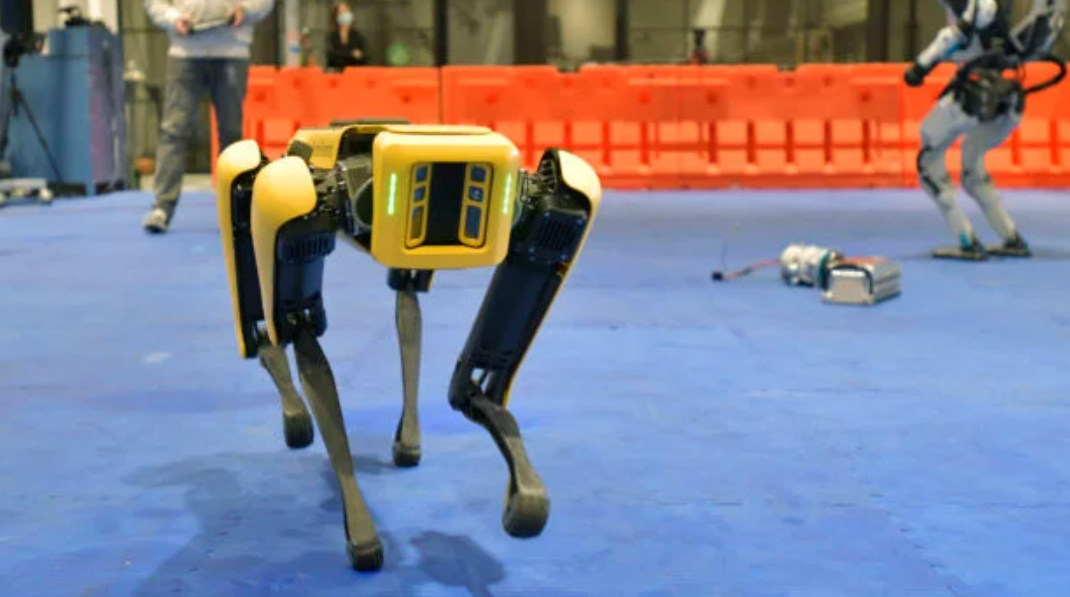
\includegraphics[width=1.0\textwidth]{figures/introduction/robot1}
\end{center}
\end{frame}
\begin{frame}[fragile]{} 
\begin{center}
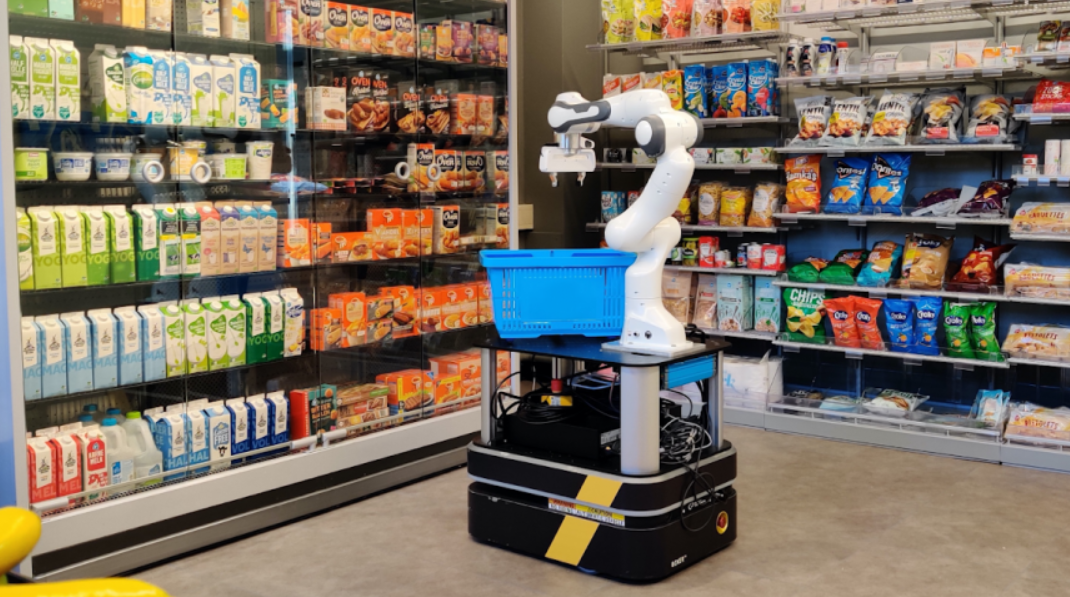
\includegraphics[width=1.0\textwidth]{figures/introduction/robot2}
\end{center}
\end{frame}
\begin{frame}[fragile]{} 
\begin{center}
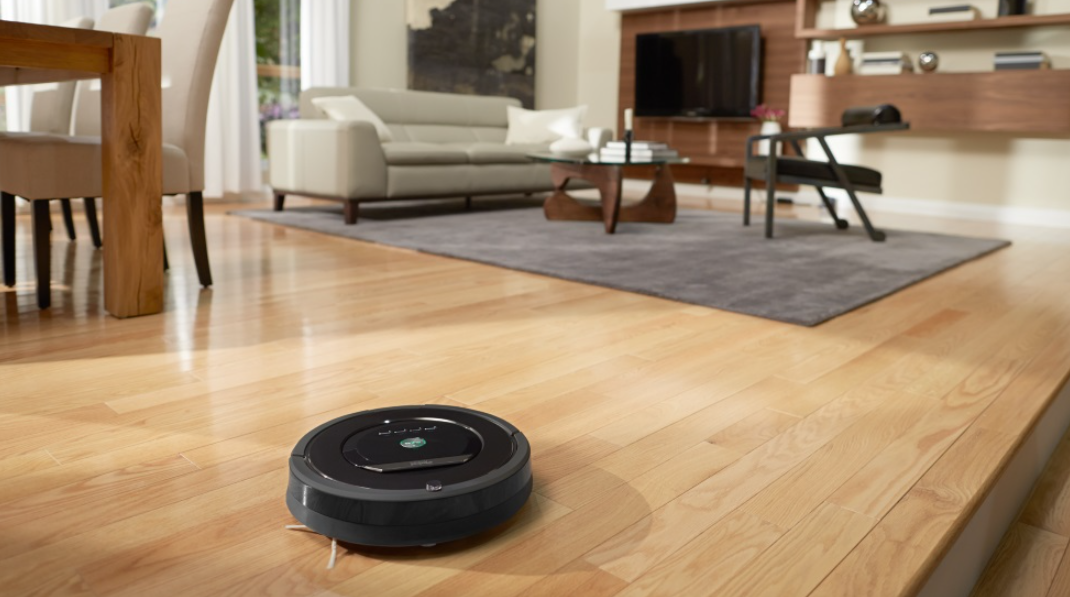
\includegraphics[width=1.0\textwidth]{figures/introduction/robot4}
\end{center}
\end{frame}
\begin{frame}[fragile]{} 
\begin{center}
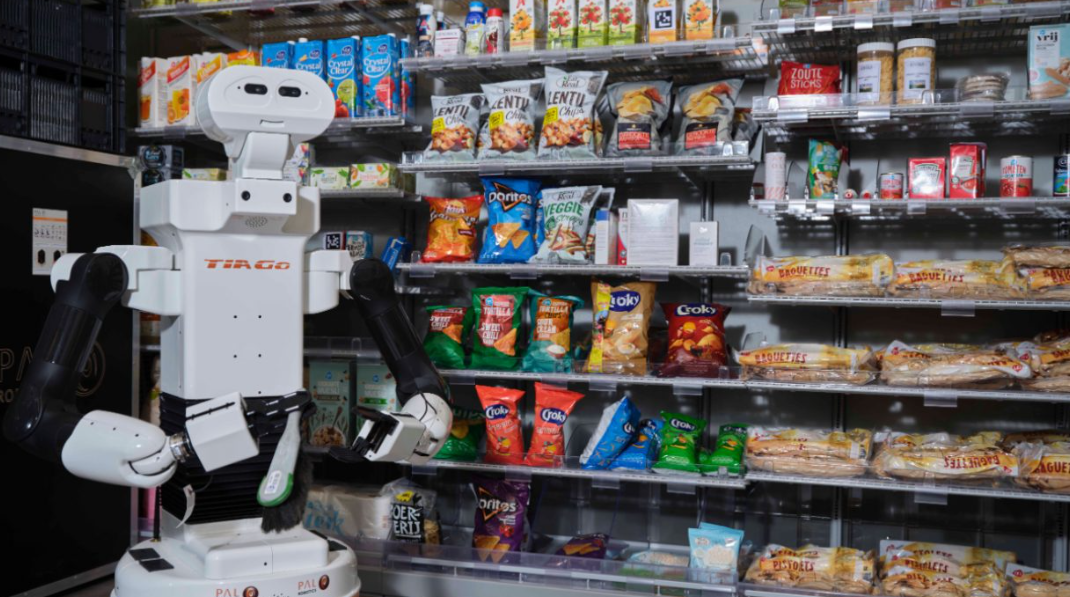
\includegraphics[width=1.0\textwidth]{figures/introduction/robot3}
\end{center}
\end{frame}

\begin{frame}[c]{Intro} 
  \begin{block}{Table of Content}
    \begin{enumerate}
      \item Introduction
      \item Required Background
      \item Proposed Method
      \item Results
      \item Conclusions
    \end{enumerate}
  \end{block}
\end{frame}

\begin{frame}[fragile]{Intro} 
\begin{itemize}
  \item Learn System Models\\\pause
  \item Navigation Among Movable Objects (NAMO)\\\pause
  \item Nonprehensile Pushing
\end{itemize}
\end{frame}

\begin{frame}[fragile]{Intro}
\large
How do learned objects' system models improve global task planning for a robot with nonprehensile push manipulation abilities over time? \bs

\textbf{Research Subquestions:}

\begin{enumerate}
    \item\small How to combine learning and planning for push and drive applications?
    \item\small How does the proposed framework compare against the state-of-the-art?
\end{enumerate}
\end{frame}

\begin{frame}[c]{Intro: Overview Proposed Method} 
  \vspace{0.3cm}
\centering
\begin{tikzpicture}[scale=1.05, every node/.style={scale=1.05}, node distance = 2cm, auto]
   
  \node [outer sep=0cm] (environment) at (0,0)  {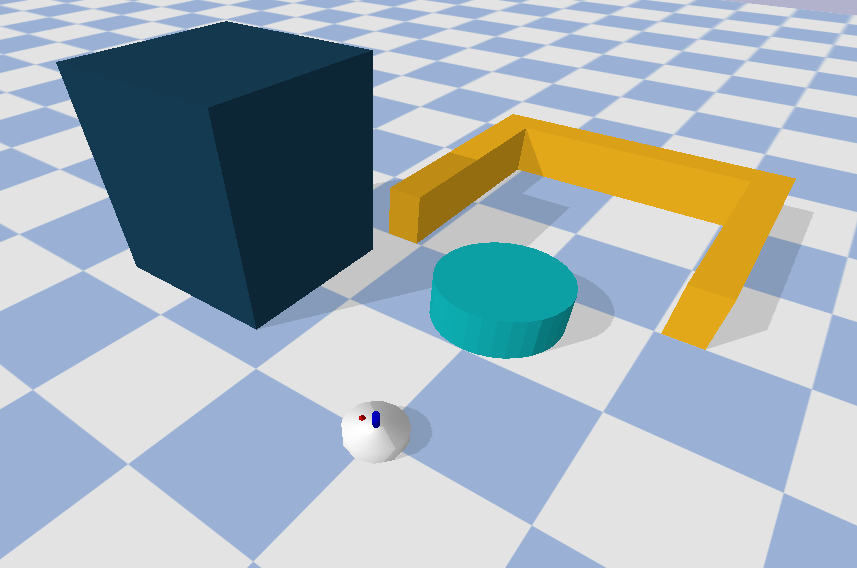
\includegraphics[width=4.6cm]{figures/introduction/blockade}}; overvew

  \draw [myEvenLighterColor,
  rounded corners=0.3cm, 
  line width=0.3cm]  
  (environment.north west) -- 
  (environment.north east) --
  (environment.south east) --
  (environment.south west) -- cycle  ;

  \node [block,
  above of=environment,
  minimum height=2cm,
  minimum width=5cm,
  node distance=4.1cm,
  outer sep=0cm] (hgraph) {Proposed Robot Framework};

  % Draw edges
  \draw[-stealth] ([yshift=0.155cm, xshift=0.4 cm]environment.north) -- node [xshift=-.05cm, right] {\shortstack[]{sensor\\measurements}}([xshift=0.4 cm]hgraph.south) ;
  \draw[-stealth] ([xshift=-0.4 cm]hgraph.south) -- node [left] {robot input}([yshift=0.155cm, xshift=-0.4 cm]environment.north) ;
  \draw[stealth-] (hgraph.west) -- node [above] {task} ++(-1, 0);

\end{tikzpicture}

\end{frame}

\begin{frame}[fragile]{Intro}
\begin{center}
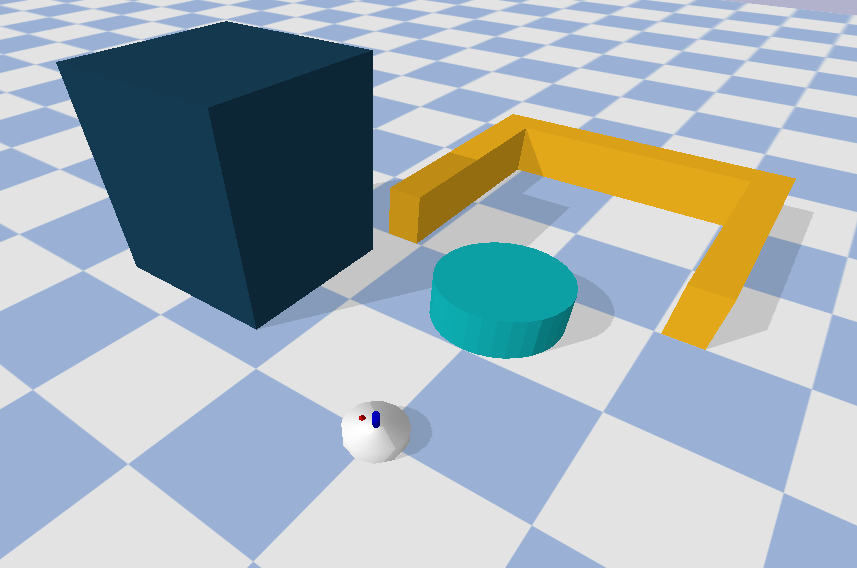
\includegraphics[width=1.0\textwidth]{figures/introduction/blockade}
\end{center}
\end{frame}


\begin{frame}[fragile]{Intro}
\begin{center}
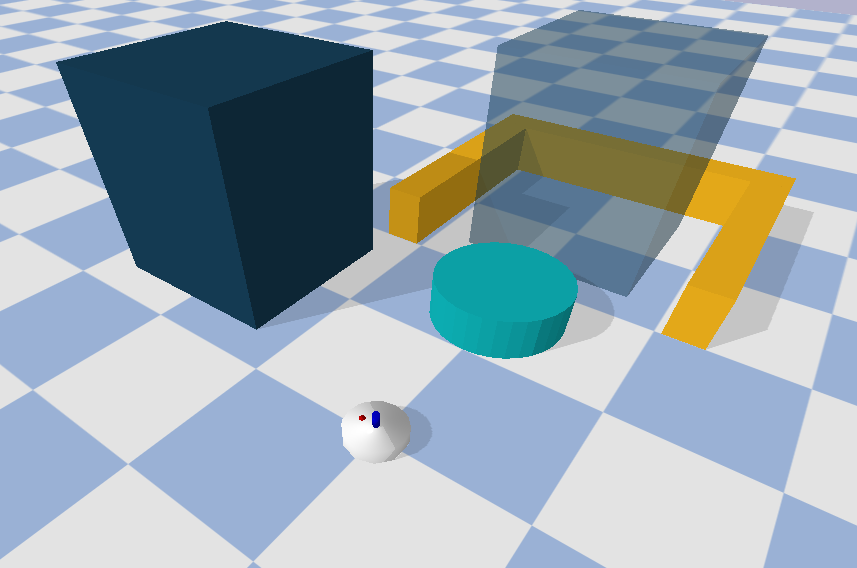
\includegraphics[width=1.0\textwidth]{figures/introduction/blockade_with_target}
\end{center}
\end{frame}

\begin{frame}[fragile]{Intro}
  \begin{center}
    \vspace{-0.2cm}
  \begin{minipage}[c]{0.8\textwidth}
    \centering
    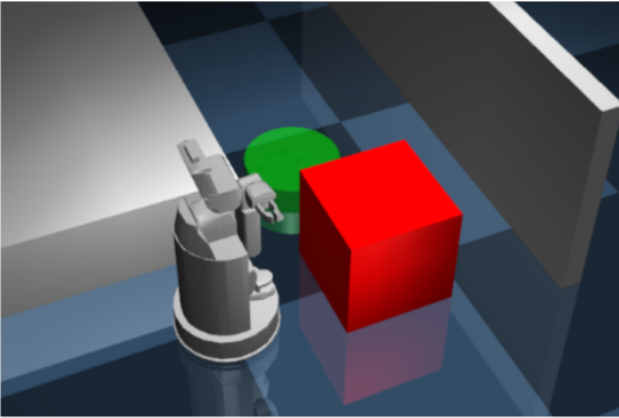
\includegraphics[width=0.9\textwidth]{figures/introduction/wang}
  \end{minipage}
  \vspace{0.3cm}
  \begin{minipage}[c]{0.5\textwidth}
     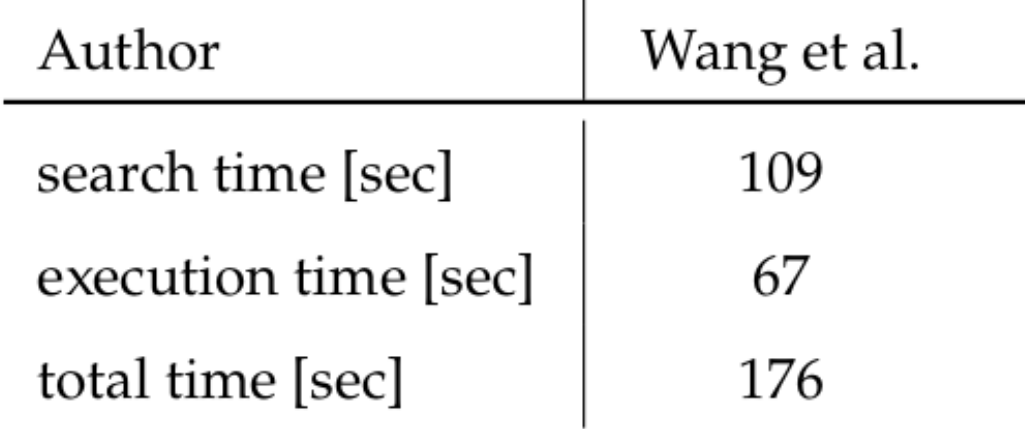
\includegraphics[width=0.8\textwidth]{figures/introduction/wang_table}
  \end{minipage}
\end{center}

\end{frame}





\begin{frame}[fragile]{Intro}
\begin{block}{Assumtions}
\begin{enumerate}
  \item \textbf{Closed-World}\pause
\item\textbf{Perfect Object Sensor}\pause
\item\textbf{Tasks are Commutative}
\end{enumerate}
\end{block}
\end{frame}
